\section{Lesson 08 --- 03/11/2026}

\subsection{Cost of a classifier}

We want to evaluate the cost of a misclassification for both positive and negative instances. A classifier is a point $(FPR, TPR)$ on the ROC plane, and its cost is
\[
  cost = FPR \cdot P(n) \cdot c(Y,n) + FNR \cdot P(p) \cdot c(N,p),
  \qquad FNR = \frac{FN}{P} = 1 - TPR.
\]

$P(n)$ and $P(p)$ are the a-priori probabilities of a negative and of a positive example. $c(Y,n)$ and $c(N,p)$ are the false-positive and false-negative costs. Once probabilities and costs are fixed, the points with the same cost lie on a line of slope
\[
  slope = \frac{P(n)\, c(Y,n)}{P(p)\, c(N,p)},
\]
so we obtain a family of parallel \g{iso-cost lines}. On the ROC plane the cost function is therefore a line, and we want to find the point of the ROC curve that is tangent to the lowest-cost line: this point is the optimal threshold for our classifier.

\begin{center}
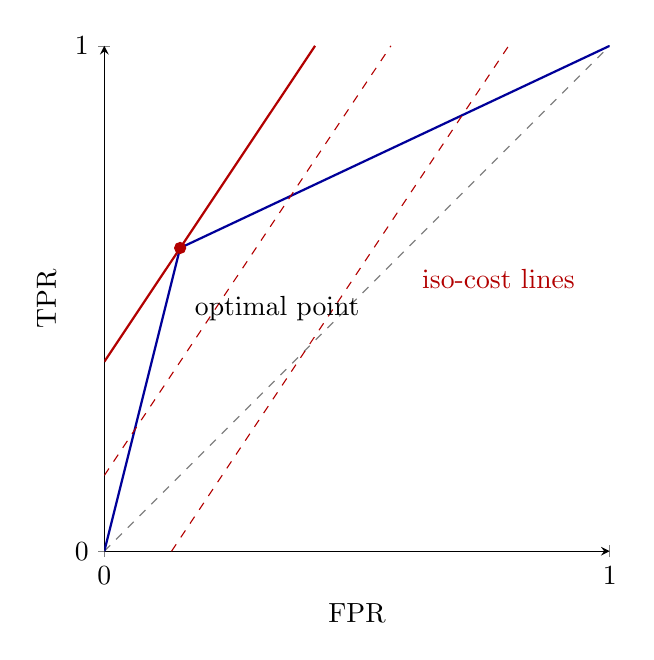
\begin{tikzpicture}
\begin{axis}[
  width=8cm, height=8cm,
  xmin=0, xmax=1, ymin=0, ymax=1,
  xlabel={FPR}, ylabel={TPR},
  xtick={0,1}, ytick={0,1},
  axis lines=left, clip=true]
  \addplot[dashed, gray] coordinates {(0,0) (1,1)};
  \addplot[thick, blue!60!black] coordinates {(0,0) (0.15,0.6) (1,1)};
  \addplot[red!70!black, dashed] coordinates {(0,0.15) (0.567,1)};
  \addplot[red!70!black, dashed] coordinates {(0.133,0) (0.8,1)};
  \addplot[red!70!black, thick] coordinates {(0,0.375) (0.417,1)};
  \addplot[only marks, mark=*, red!70!black] coordinates {(0.15,0.6)};
  \node[right] at (axis cs:0.16,0.48) {optimal point};
  \node[red!70!black, above] at (axis cs:0.78,0.5) {iso-cost lines};
\end{axis}
\end{tikzpicture}
\end{center}

\subsection{Estimating Classifier Accuracy}

To decide which classifier is the best for our application domain we can't base our evaluation on only one trial, also because we can have different results depending on the training and test sets (we have only one labelled dataset). The solution is to repeat the evaluation under different partitions of training and test sets, and then average the results. After this process we will have a statistical distribution of results. How can we compare distributions? We can use the mean and the standard deviation of the results, but we need to be careful because the sample mean and the sample standard deviation are also random variables, so we need to estimate a confidence interval (this is what Stea said and I think is better). For prof. Marcelloni we need to perform some statistical tests to compare the distributions, for example the t-test.

Some simple methods based on repeated train/test partitions are the \g{holdout method} and \g{random subsampling}.

\begin{algorithm}[H]
\caption{Holdout method}
\KwIn{dataset $D$, training fraction (e.g.\ $2/3$)}
\KwOut{accuracy estimate}
Randomly partition $D$ into two independent sets: a training set $D_{train}$ (e.g.\ $2/3$ of $D$) and a test set $D_{test}$ (e.g.\ $1/3$ of $D$)\;
Build the model $M$ on $D_{train}$\;
Estimate the accuracy of $M$ on $D_{test}$\;
\end{algorithm}

\begin{algorithm}[H]
\caption{Random subsampling}
\KwIn{dataset $D$, number of repetitions $k$}
\KwOut{accuracy estimate}
\For{$i = 1$ \KwTo $k$}{
  Apply the holdout method on a new random partition of $D$, obtaining the accuracy $acc_i$\;
}
\Return{$\frac{1}{k}\sum_{i=1}^{k} acc_i$}\;
\end{algorithm}

\g{k-fold Cross-validation}:
We start by randomly partitioning the dataset into $k$ mutually exclusive subsets of approximately equal size (\g{folds}) $D_1, \dots, D_k$. At each iteration $i$ we use the fold $D_i$ as test set and the remaining $k-1$ folds as the training set. The accuracy is the average of the $k$ estimates. Usually $k$ equals 10 because with 10 iterations we can have some statistical significance.

\subsubsection{Null hypothesis and paired comparison}

To compare two classifiers $M_1$ and $M_2$ we use paired samples: both classifiers are evaluated on the same $k$ folds. At each fold $i$ we compute $err(M_1)_i$ and $err(M_2)_i$ and we analyze the paired differences
\[
  d_i = err(M_1)_i - err(M_2)_i.
\]
Pairing reduces the variability due to different partitions. The \g{null hypothesis} is that the two classifiers have the same error on average, i.e.\ the expected difference is zero:
\[
  H_0: \mu_d = 0.
\]
The test assumes that the differences are approximately normally distributed and that the variances of the two populations are not reliably different. If $H_0$ is rejected, the observed difference is statistically significant and we choose the model with the lower estimated error rate.

\subsection{Paired t-test}

The paired t-test is a formal statistical test for the mean difference in cross-validation errors.

\begin{algorithm}[H]
\caption{Paired t-test}
\KwIn{errors $err(M_1)_i$, $err(M_2)_i$ for $i = 1,\dots,k$ on the same folds; significance level $\alpha$}
\KwOut{reject $H_0$ or not}
Compute the paired differences $d_i = err(M_1)_i - err(M_2)_i$, $i = 1,\dots,k$\;
Estimate the mean difference $\bar d = \frac{1}{k}\sum_{i=1}^{k} d_i$\;
Compute the sample variance of the differences $s_d^2 = \frac{1}{k-1}\sum_{i=1}^{k} (d_i - \bar d)^2$\;
Compute the statistic $t = \dfrac{\bar d}{s_d / \sqrt{k}}$\;
Set the degrees of freedom $df = k-1$, which determine the shape of the t-distribution\;
\eIf{$|t| > t_{1-\alpha/2,\,k-1}$}{reject $H_0$ (the mean difference is statistically different from zero)}{do not reject $H_0$ (the observed difference may be due to chance)}
\end{algorithm}

For example, for $k = 10$ and $\alpha = 0.05$ the critical value is $t_{0.975,\,9} \approx 2.262$.

\begin{remark}
In $k$-fold cross-validation the $k$ estimates are not fully independent, because the training sets overlap, so the simple paired t-test can underestimate the variance. For a more rigorous comparison one can use the corrected resampled t-test, the $5\times 2$cv test, or repeated/nested cross-validation protocols. Moreover, failing to reject $H_0$ does not mean that the two classifiers are equivalent: it only means that there is insufficient statistical evidence to conclude that their expected performances differ.
\end{remark}
